%% ****** Start of file template.aps ******%
%%
%%
%%   This file is part of the APS files in the REVTeX 4 distribution.
%%   Version 4.0 of REVTeX, August 2001
%%
%%
%%   Copyright (c) 2001 The American Physical Society.
%%
%%   See the REVTeX 4 README file for restrictions and more information.
%%
%
% This is a template for producing manuscripts for use with REVTEX 4.0
% Copy this file to another name and then work on that file.
% That way, you always have this original template file to use.
%
% Group addresses by affiliation; use superscriptaddress for long
% author lists, or if there are many overlapping affiliations.
% For Phys. Rev. appearance, change preprint to twocolumn.
% Choose pra, prb, prc, prd, pre, prl, prstab, or rmp for journal
%  Add 'draft' option to mark overfull boxes with black boxes
%  Add 'showpacs' option to make PACS codes appear
%  Add 'showkeys' option to make keywords appear
% \documentclass[aps,prl,preprint,groupedaddress]{revtex4}
%\documentclass[aps,prl,preprint,superscriptaddress]{revtex4}
\documentclass[aps,prl,twocolumn,groupedaddress]{revtex4}

\usepackage{amsmath,pdfpages}

% You should use BibTeX and apsrev.bst for references
% Choosing a journal automatically selects the correct APS
% BibTeX style file (bst file), so only uncomment the line
% below if necessary.
%\bibliographystyle{apsrev}

\begin{document}

%\preprint{}

%Title of paper
\title{Anomalous Dispersion at ELANEX, CHERNEAR}

\author{Joel Frederico}
%\email[]{Your e-mail address}
%\homepage[]{Your web page}
%\thanks{}
\altaffiliation{Stanford University}
\affiliation{SLAC Nat'l Accelerator Lab}

%Collaboration name if desired (requires use of superscriptaddress
%option in \documentclass). \noaffiliation is required (may also be
%used with the \author command).
%\collaboration can be followed by \email, \homepage, \thanks as well.
%\collaboration{}
%\noaffiliation

\date{\today}

\begin{abstract}
Dispersion at the lanex screen is anomalous.  The pinch in the butterfly for different quad settings doesn't reflect the calibrated dispersion.  Possible explanations are investigated.  Lessons learned and implemented.
\end{abstract}

\maketitle

\section{Intro}

If you look at the pinch location in the butterfly for different quad settings on Nov.~8, 2013, the pinch is not at the correct energy location.  The dispersion at the lanex screen is expected to be 62~mm, and with a resolution of ~10 $\mu$m/px, the offset of the pinch can be calculated.  This first hinted that the dispersion was wrong.  Rather than go through a calculation of where offsets are to be expected, it is more compelling to calculate the dispersion seen.

There are only 2 independent variables: the calibrated resolution of the camera at ~10 $\mu$/px, which is well-understood per Sebastien; and the matlab function that changed the energy focus at the lanex screen for each step, which I am assured is well-understood per Sebastien and Erik.

The third variable- the pinch location/energy calibration at the lanex screen- is suspect at the moment.  There is one additional assumption made- that the pinch location is actually the location of the energy that is in focus by the quads.  It is possible that this is not true, perhaps through a waist-energy correlation, although I don't think that's the most likely explanation.  One of the best explanations is that there is additional y-dispersion due to tuning/upstream effects.

I will do my best to explore all of these possibilities.

\section{Expected Dispersion}

Per pencil beam/spectrometer magnet scans, the expected dispersion at the near cherenkov wafers is 62mm.  The dispersion upstream can be given by:
\begin{align}
	\eta_{lanex} &= \eta_{cher} \frac{\textrm{distance, spec mag to lanex}}{\textrm{distance, spec mag to cher}}\\
	&= \textrm{62mm} \frac{\textrm{9.8m}}{\textrm{10.3m}}\\
	&\approx \textrm{57.5mm}
	\label{}
\end{align}

\section{Measuring Dispersion}

As mentioned previously, the dispersion can be calculated assuming that the quadrupole values are focused correctly and the pinch is representative of the location of the energy in focus.  A rough ROI was selected to track the pinch.  Each ROI was sliced in y in 2-px increments.  Each slice was then fit with a gaussian.  The slices were compiled and fit with a line to recover the dispersion.  The dispersion measured was $\eta_y\approx-23.9$mm.  There is a difference of roughly 30mm which has to be accounted for.

\begin{figure}
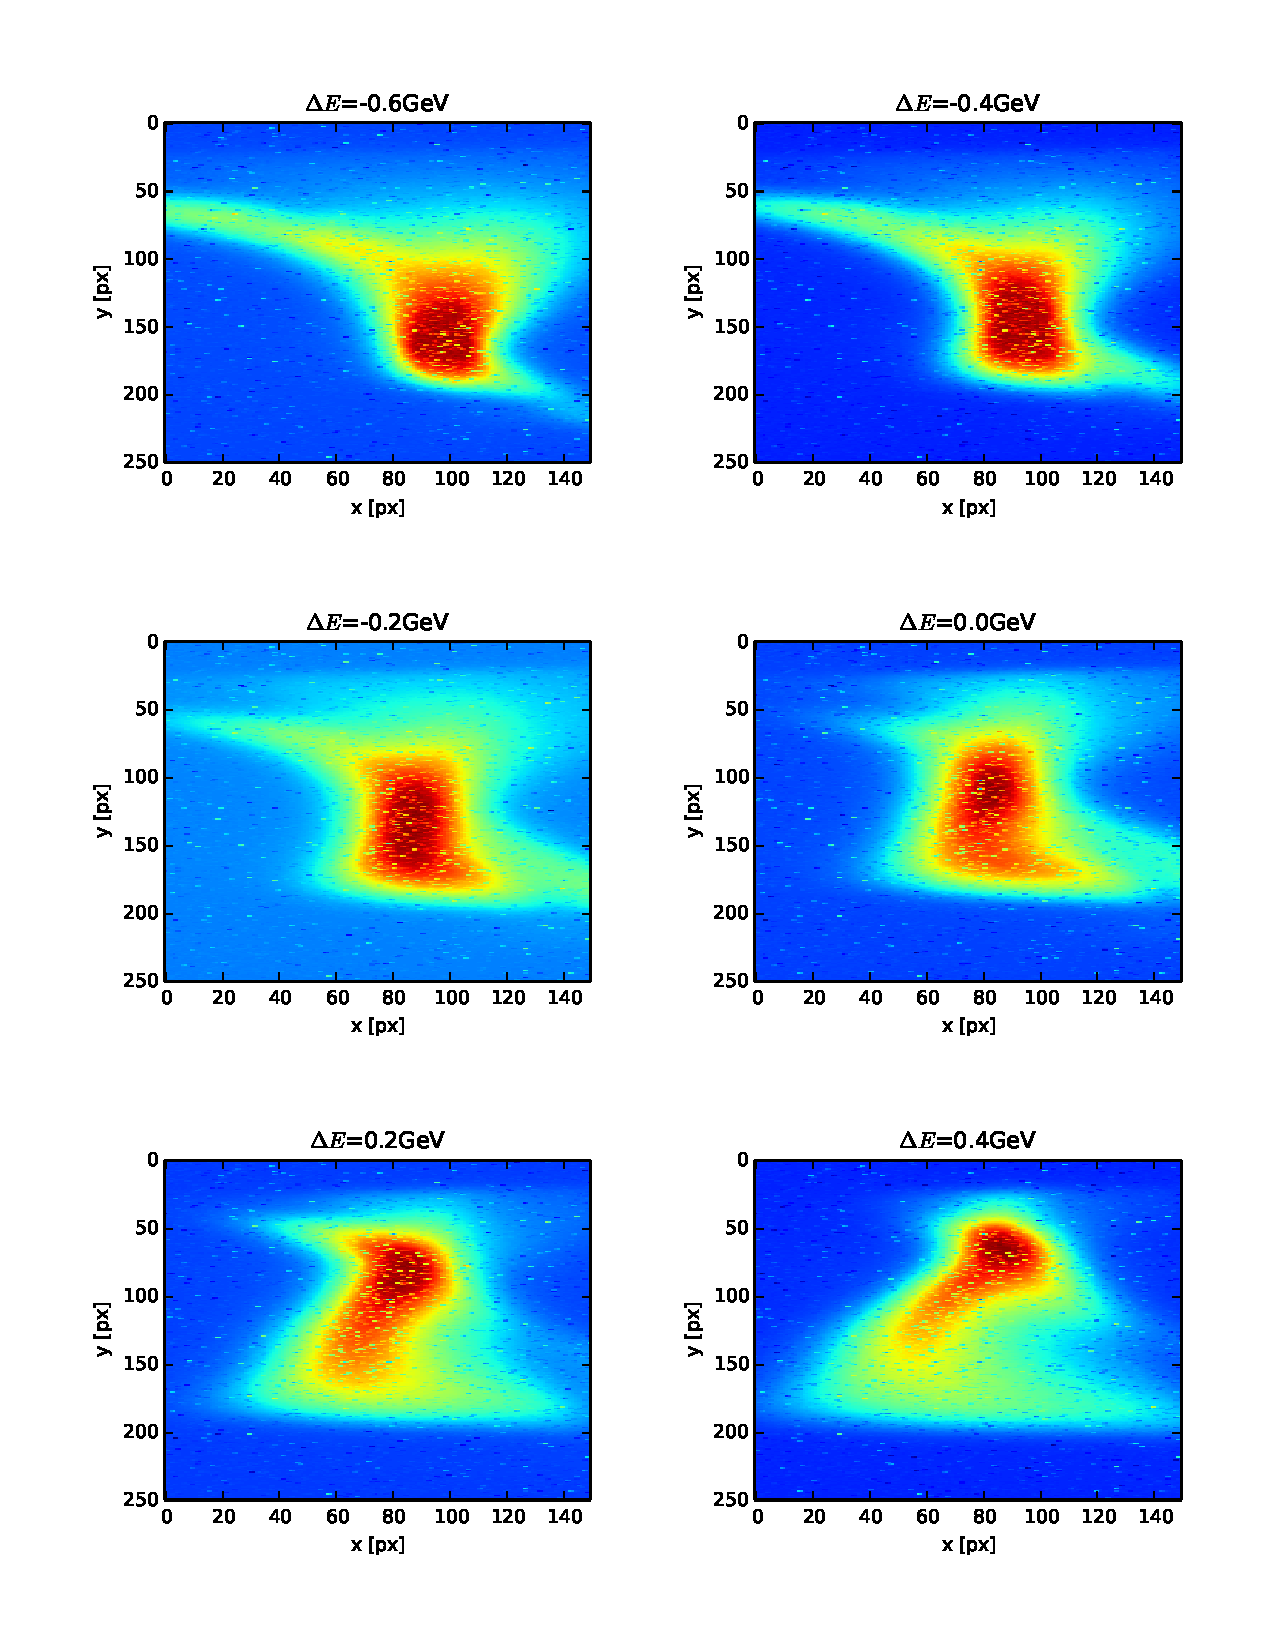
\includegraphics[scale=0.3,page=1]{output.pdf}
\caption{Shots are -0.6Gev, -0.4GeV, -0.2GeV, 0GeV, 0.2GeV, 0.4GeV, in the order you'd expect.}
\end{figure}

\begin{figure}
\includegraphics[scale=0.3,page=2]{output.pdf}
% \caption{Shots are -0.6Gev, -0.4GeV, -0.2GeV, 0GeV, 0.2GeV, 0.4GeV, in the order you'd expect.}
\end{figure}

% \begin{figure}
% \includegraphics{}%
% \caption{\label{}}
% \end{figure}


% Create the reference section using BibTeX:
% \bibliography{basename of .bib file}

\end{document}
%
% ****** End of file template.aps ******


